\section{Statistical compression I: Huffman coding}
\label{sec:01}

\subsection{Prefix codes}

\paragraph{Memoryless sources}

We have some data that we wish to encode. It could be anything: Spoken English, Data from a digital camera sensor, DNA string, etc.

We model our data as coming from a memoryless source $X$. We imagine that symbols are emitted at random according to the probability distribution of $X$. In other words, we view our data as a random string $X_1, X_2, \dots$ over some alphabet $\mathcal{X}$. Our memoryless assumption is that those form a sequence of independent identically distributed (i.i.d.) random variables: $X_i \sim X$ for all $i$.

More concretely, for any $x \in \mathcal{X}$ and any $i$, the probability 
\[
\probability(X_i = x)
\]
is independent of $i$, and of all previous or future emitted symbols.

Note that this is not always a valid assumption. We will look into source modelling into more detail in the next lectures.



\paragraph{The coding problem}


We have a source emitting symbols in $\mathcal{X} = \{x_1, \dots, x_n\}$ with respective probabilities  $\{p_1, \dots, p_n\}$.


Question: If  $\mathcal{D}$ is an alphabet of  $D$ code symbols, how can we encode the source symbols using code words (finite strings of code symbols) as economically as possible?

Formally: a \Define{source code} is a map $C : \mathcal{X} \to \mathcal{D}^*$
where  $\mathcal{D}^*$     is the set of all finite strings of symbols in  $\mathcal{D}$.

The words $C(x)$ are called the \Define{codewords}, and the integers $|C(x)|$ (the length of $C(x)$) are the \Define{word lengths}.


We can extend the code to messages as follows. A \Define{message} is any finite string of source symbols $m = m_1 \dots m_k \in \mathcal{X}^*$ and its encoding is the obvious concatenation 
\[
    C(m) = C(m_1) C(m_2) \dots C(m_k).
\]



\paragraph{Prefix codes}


A code $C$ is \Define{uniquely decodable} (a.k.a. uniquely decipherable) if every finite string in $\mathcal{D}^*$ is the image of at most one message. 

A prefix of a word $w = w_1 \dots w_k \in \mathcal{D}^*$ is any word of the form $w_1 \dots w_l$ for some $0 \le l \le k$ (for $l=0$, we obtain the empty word). A code is \Define{prefix} (a.k.a. instantaneous or prefix-free) if there are no two distinct source symbols $x, y \in \mathcal{X}$ such that $C(x)$ is a prefix of  $C(y)$         .

\begin{theorem}
A prefix code is uniquely decodable.
\end{theorem}

\begin{proof}
Let $C$ be a prefix code, and let $w = C(m)$ for some message $m = m_1 \dots m_k \in \mathcal{X}^*$. We give a decoding algorithm which, given $w$, determines $m$. Let $w = w_1 \dots w_l$.

Let $i$ be the smallest integer such that $w_1 \dots w_i$ is a codeword, say $w_1 \dots w_i = C(x)$. Then the $m_1 = x$. Indeed, if $m_1 = y \ne x$, then $C(x)$ is a prefix of $C(y)$, which is a contradiction. Then repeat this step, beginning with $w_{i+1}$ and hence determining $m_2$, and so on until $w$ is empty.
\end{proof}

\begin{example}
Let $\mathcal{X} = \{a, b, c, d, e\}$, $\mathcal{D} = \{0,1\}$ and 
\begin{align*}
    C(a) &= 01\\
    C(b) &= 100\\
    C(c) &= 101\\
    C(d) &= 1101\\
    C(e) &= 1111.
\end{align*}

Suppose we need to decode the word $C(m) = w = 10010111011111100101$. We proceed as follows. We read the word until we reach a codeword:
\begin{align*}
    w_1 &= 1\\
    w_1 w_2 &= 10\\
    w_1 w_2 w_3 &= 100 = C(b). 
\end{align*}
Therefore $m_1 = b$. We continue until we reach a codeword:
\begin{align*}
    w_4 &= 1\\
    w_4 w_5 &= 10\\
    w_4 w_5 w_6 &= 101 = C(c). 
\end{align*}
Therefore $m_2 = c$. And so on... Exercise \ref{exercise:prefix} asks you to finish this simple example.
\end{example}




\subsection{Huffman codes}


\paragraph{Compact codes}

Our main aim is to design codes where the typical length of messages is reduced dramatically. The basic idea is to assign short codewords to more frequent symbols and longer codewords to less frequent ones.


More formally, the \Define{average length} (a.k.a. expected length) of the code is 
\[
    L(C) = \expectation( |C(X)| ) = \sum_{x \in \mathcal{X}} |C(x)| \probability(X = x).
\]

A code is \Define{compact} (for a given source $X$) if it is uniquely decodable and it minimises the average length of codewords over all uniquely decodable codes.


\begin{theorem}
A uniquely decodable code with prescribed word lengths exists if and only if a prefix code with the same word lengths exists.
\end{theorem}

We shall prove this result in Lecture \ref{sec:35}.

\begin{corollary}
For any source $X$, there is a compact prefix code for $X$.
\end{corollary}


\paragraph{Binary Huffman code}


The key is to construct a tree where the leaves correspond to the symbols in  $\mathcal{X}$ and the paths from the root to the leaves give the codewords.

The tree is constructed iteratively. Suppose $\mathcal{X} = \{x_1, \dots, x_n\}$ with $p_1 \ge p_2 \ge  \dots \ge p_{n-1} \ge p_n$. Then merge $x_{n-1}$ and $x_n$ into a new symbol, say $x_{n-1, n}$ with probability $p_{n-1} + p_n$, and let $x_{n-1}$ and $x_n$ be the children of $x_{n-1, n}$ on the tree. Label the edges from $x_{n-1, n}$ to its children as $0$ and $1$, respectively. Repeat for the new source $X^{(1)} = \{x_1, \dots, x_{n-2}, x_{n-1, n} \}$ (making sure to order the symbols in non-decreasing probability). Repeat until the final source $X^{(n-1)}$ only has one symbol left with probability $1$; that symbol is the root of the tree. 

Once the tree is built, read off the labels on the path from the root to a leaf to get the corresponding codeword.

\begin{example} \label{example:huffman}
Let $X$ with respective probabilities $a: 0.4, b: 0.2, c: 0.15, d:0.15, e:0.1$.

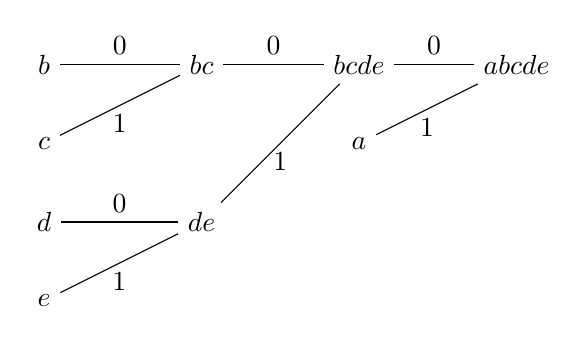
\begin{tikzpicture}[xscale=2]
    %\node (a0) at (0,4) {$a$}; %0.4
    %\node (b0) at (0,3) {$b$}; %0.2
    %\node (c0) at (0,2) {$c$}; %0.15
    \node (d0) at (1,2) {$d$}; %0.15
    \node (e0) at (1,1) {$e$}; %0.1
    
    %\node (a1) at (1,4) {$a$}; %0.4
    %\node (de1) at (1,3) {$de$}; %0.25
    \node (b1) at (1,4) {$b$}; %0.2
    \node (c1) at (1,3) {$c$}; %0.15
    
    %\node (a2) at (2,4) {$a$}; %0.4
    \node (bc2) at (2,4) {$bc$}; %0.35
    \node (de2) at (2,2) {$de$}; %0.25

    \node (bcde3) at (3,4) {$bcde$}; %0.6
    \node (a3) at (3,3) {$a$}; %0.4

    \node (abcde4) at (4,4) {$abcde$}; %1

\draw (de2) -- node[above] {$0$} ++(d0);
\draw (de2) -- node[below] {$1$} ++(e0);

\draw (bc2) -- node[above] {$0$} ++(b1);
\draw (bc2) -- node[below] {$1$} ++(c1);

\draw (bcde3) -- node[above] {$0$} ++(bc2);
\draw (bcde3) -- node[below] {$1$} ++(de2);

\draw (abcde4) -- node[above] {$0$} ++(bcde3);
\draw (abcde4) -- node[below] {$1$} ++(a3);


\end{tikzpicture}

The code is then
\begin{align*}
    C(a) &= 1\\
    C(b) &= 000\\
    C(c) &= 001\\
    C(d) &= 010\\
    C(e) &= 011
\end{align*}
The average length is then $2.2$ bits per symbol.
\end{example}


Note that there is no need for general tie-breaking rules. Indeed, different merges may yield different codes, and maybe even different code lengths, but always the same expected length. Similarly, the assignment of $0$ or $1$ does not change the code lengths.



\paragraph{Huffman codes are compact} Clearly, Huffman codes are prefix. The proof that they are compact is by induction on the number of symbols and omitted. It can be found in \cite[Section 5.8]{CT06}.


\paragraph{Non-binary Huffman codes}

Huffman codes can be extended to non-binary alphabets: If we have an alphabet of $D$ characters, we group the $D$ least likely symbols at each stage of reducing the source. When expanding the code we append each of the $D$ characters to one of the least likely symbols' codewords.

We must end up with exactly $D$ symbols in the final source, so we may need to pad the original source up to $D+k(D-1)$ by adding symbols of probability $0$.

\subsection{See further}

\paragraph{Codes and Automata} The mathematical theory of uniquely decodable codes is reviewed in \cite{BPR10}, where they are simply referred to as codes. The language generated by a prefix code can be recognised by very a simple deterministic finite automaton; in fact, the relation between codes and automata is very deep and explored throughout the book. Note that this book hardly talks about data compression!

\paragraph{Canonical Huffman codes} As we shall see in Exercise \ref{exercise:huffman_unequal_lengths}, there can be several different Huffman trees for the same source. However, there is always a so-called canonical Huffman tree (and hence code) with a special shape that can be easily computed; see \cite[3.2.2]{Say12}. We shall encounter a similar idea in Lecture \ref{sec:35}.

\paragraph{Adaptive Huffman coding} Huffman coding is based on a source $X$ with given probabilities. In general, the probability of an element is computed by its relative frequency in the message; for instance, if the message has 100 characters, 34 of them are ``e'', then the probability of ``e'' is 34\%. Computing those probabilities then requires scanning the whole document before building the tree. Adaptive Huffman coding, on the other hand, builds the Huffman tree as the document is scanned, making small updates (if any) each time a new character is scanned.

\subsection{Exercises}

\begin{exercise} \label{exercise:not_prefix}
Let $\mathcal{X} = \{x_1, \dots, x_q\}$ for $q \ge 2$. Give a binary code $C : \mathcal{X} \to \{0,1\}^*$ that is uniquely decodable but neither prefix nor suffix.
\end{exercise}

\begin{exercise} \label{exercise:prefix}
Finish the example of decoding a prefix code.
\end{exercise}

\begin{exercise} \label{exercise:decoding_prefix}
How could you make the decoding algorithm of prefix codes more efficient? Would you use that modification for decoding Huffman codes? How would you include the decision problem: given $w \in \mathcal{D}^*$, determine whether $w$ is a codeword.
\end{exercise}

\begin{exercise} \label{exercise:huffman}
Construct a binary Huffman code for $X$ with probabilities $0.5, 0.2, 0.15, 0.1, 0.05$. What is the average length, and how does it compare with the one in Example \ref{example:huffman}?
\end{exercise}

\begin{exercise} \label{exercise:huffman_unequal_lengths}
Let $X$ have probabilities $(1/3, 1/3, 1/4, 1/{12})$. Show that, depending on how you merge, the binary Huffman coding procedure may lead to different code lengths, namely $(2,2,2,2)$ or $(1,2,3,3)$. Verify that the average length remains the same, though.
\end{exercise}



